\documentclass[handout,nooutcomes]{ximera}
\usepackage{booktabs}
%% handout
%% space
%% newpage
%% numbers
%% nooutcomes

\renewcommand{\outcome}[1]{\marginpar{\null\vspace{2ex}\scriptsize\framebox{\parbox{0.75in}{\begin{raggedright}P\arabic{problem} Outcome: #1\end{raggedright}}}}}

\renewenvironment{freeResponse}{
\ifhandout\setbox0\vbox\bgroup\else
\begin{trivlist}\item[\hskip \labelsep\bfseries Solution:\hspace{2ex}]
\fi}
{\ifhandout\egroup\else
\end{trivlist}
\fi}

\newcommand{\RR}{\mathbb R}
\renewcommand{\d}{\,d}
\newcommand{\dd}[2][]{\frac{d #1}{d #2}}
\renewcommand{\l}{\ell}
\newcommand{\ddx}{\frac{d}{dx}}
\everymath{\displaystyle}
\newcommand{\dfn}{\textbf}
\newcommand{\eval}[1]{\bigg[ #1 \bigg]}


\title{Breakout Session 5: To infinity using limits}  

\begin{document}
\begin{abstract}
  \textbf{A look back:} In the previous (January 21, 2016) Breakout Session you practiced the fundamental techniques of evaluating limits using pen and paper.
  Evaluating limits ``by hand'' essentially consists of two components: identifying the form of the limit and reshaping to transform a harder limit to an easier limit.

  \textbf{Overview:} In today's (January 26, 2016) Breakout Session you will practice evaluating limits to locate horizontal and vertical asymptotes.
  This skill also consists of two components: identifying the form of the limit and using the form to determine rapid growth, rapid decay, or end behavior.

  \textbf{A look ahead:} In the next (January 28, 2016) Breakout Session you will investigate a special class of functions defined in terms of limits.
\end{abstract}
\maketitle

\section{Learning Outcomes}
\label{section:learning-outcomes}
The following outcomes are \emph{not an exhaustive} list of the skills you will need to develop and integrate for demonstration on quizzes and exams.
This list is meant to be a starting point for conversation (with your Lecturer, Breakout Session Instructor, and fellow learners) for organizing your knowledge and monitoring the development of your skills.

% \subsection*{Outcomes for infinite limits}
% \label{section:learning-outcomes-infinite-limits}
\begin{itemize}
  \item 
    Recognize when a limit is indicating there is a vertical asymptote.

  \item
    Evaluate the limit as $x$ approaches a point where there is a vertical asymptote.

  \item
    Match graphs of functions with their equations based on vertical asymptotes.

  \item  
    Discuss what it means for a limit to equal $\pm\infty$.

  \item 
    Define a vertical asymptote.

  \item
    Understand the relationship between limits and vertical asymptotes.
\end{itemize}

% \subsection*{Outcomes for limits at infinity} 
\begin{itemize}
  \item
    Calculate the limit as $x$ approaches $\pm\infty$ of common functions algebraically.

  \item
    Decide whether a form is determinate or indeterminate. 

  \item
    Find the limit as $x$ approaches $\pm\infty$ from a graph. 

  \item 
    Discuss why infinity is not a number. 
\end{itemize}
\newpage

\begin{problem}
  \label{problem:warmup-for-forms}
  For each of the following statements, produce a function $f$ such that it satisfies the stated conditions.
  \begin{itemize}
    \item[(a)]
      The limit of $f$ as $x$ approaches 4 has the form $\frac{0}{0}$ and the limit exists as a finite number, that is, 
      \[
        \lim_{x \to 4} \underbrace{f(x)}_{\text{form $0/0$}} = L,
      \]
      where $L$ is a real number.

    \item[(b)]
      The limit of $f$ as $x$ approaches 4 has the form $\frac{0}{0}$ and the limit does not exist and is infinity, that is,
      \[
        \lim_{x \to 4} \underbrace{f(x)}_{\text{form $0/0$}} = \infty.
      \]

    \item[(c)]
      The (two-sided) limit of $f$ as $x$ approaches 4 does not exist and is infinity, that is,
      \[
        \lim_{x \to 4} f(x) = \infty.
      \]

    \item[(d)]
      The (left-sided) limit of $f$ as $x \to 4^-$ does not exist and is infinity, while the (right-sided) limit of $f$ as $x \to 4^+$ does not exist and is negative infinity, that is, $\lim_{x \to 4^-} f(x) = \infty$ and $\lim_{x \to 4^+} f(x) = -\infty$.
  \end{itemize}
\end{problem}

\begin{problem}
  \label{problem:evaluate-infinite-limits}
  Evaluate each of the following limits or say that the limit does not exist.
  If a limit does not exist, explain why.
  \begin{itemize}
    \item[(a)]
      $\displaystyle \lim_{x \to 3} \frac{x^2 - 3}{x^2 - x - 6}$

    \item[(b)]
      $\displaystyle \lim_{x \to 5} \frac{x^2 + 6}{x^2 - 3x - 10}$

    \item[(c)]
      $\displaystyle \lim_{x \to 1} \frac{4-x}{x^2 - 2x + 1}$

    \item[(d)]
      $\displaystyle \lim_{x \to 3} \frac{x^2 - 2x - 3}{\sqrt{x+1} - 2}$

    \item[(e)]
      $\displaystyle \lim_{x \to 0^+} x \cdot \sin(\ln(x))$.

    \item[(f)]
      $\displaystyle \lim_{x \to 2^-} \frac{\ln(x)}{x - 2}$.
  \end{itemize}  
\end{problem}

\begin{problem}
  \label{problem:evaluate-infinite-limits-AU15-exam1}
    Without using a graphing utility, match each function in 1--6 with the graphs of functions in A--F:
  \begin{enumerate}
    \item
      The function $f$ defined by $\displaystyle f(x) = \frac{x}{x^2 + 1}$.

    \item 
      The function $g$ defined by $\displaystyle g(t) = \frac{t}{t^2 -1}$.

    \item 
      The function $h$ defined by $\displaystyle h(w) = \frac{1}{w^2 -1}$.

    \item 
      The function $a$ defined by $\displaystyle a(u) = \frac{u}{(u-1)^2}$.

    \item 
      The function $s$ defined by $\displaystyle s(z) = \frac{1}{(z-1)^2}$.

    \item
      The function $r$ defined by $\displaystyle r(v) = \frac{v}{v+1}$.
  \end{enumerate}
  \begin{center}
    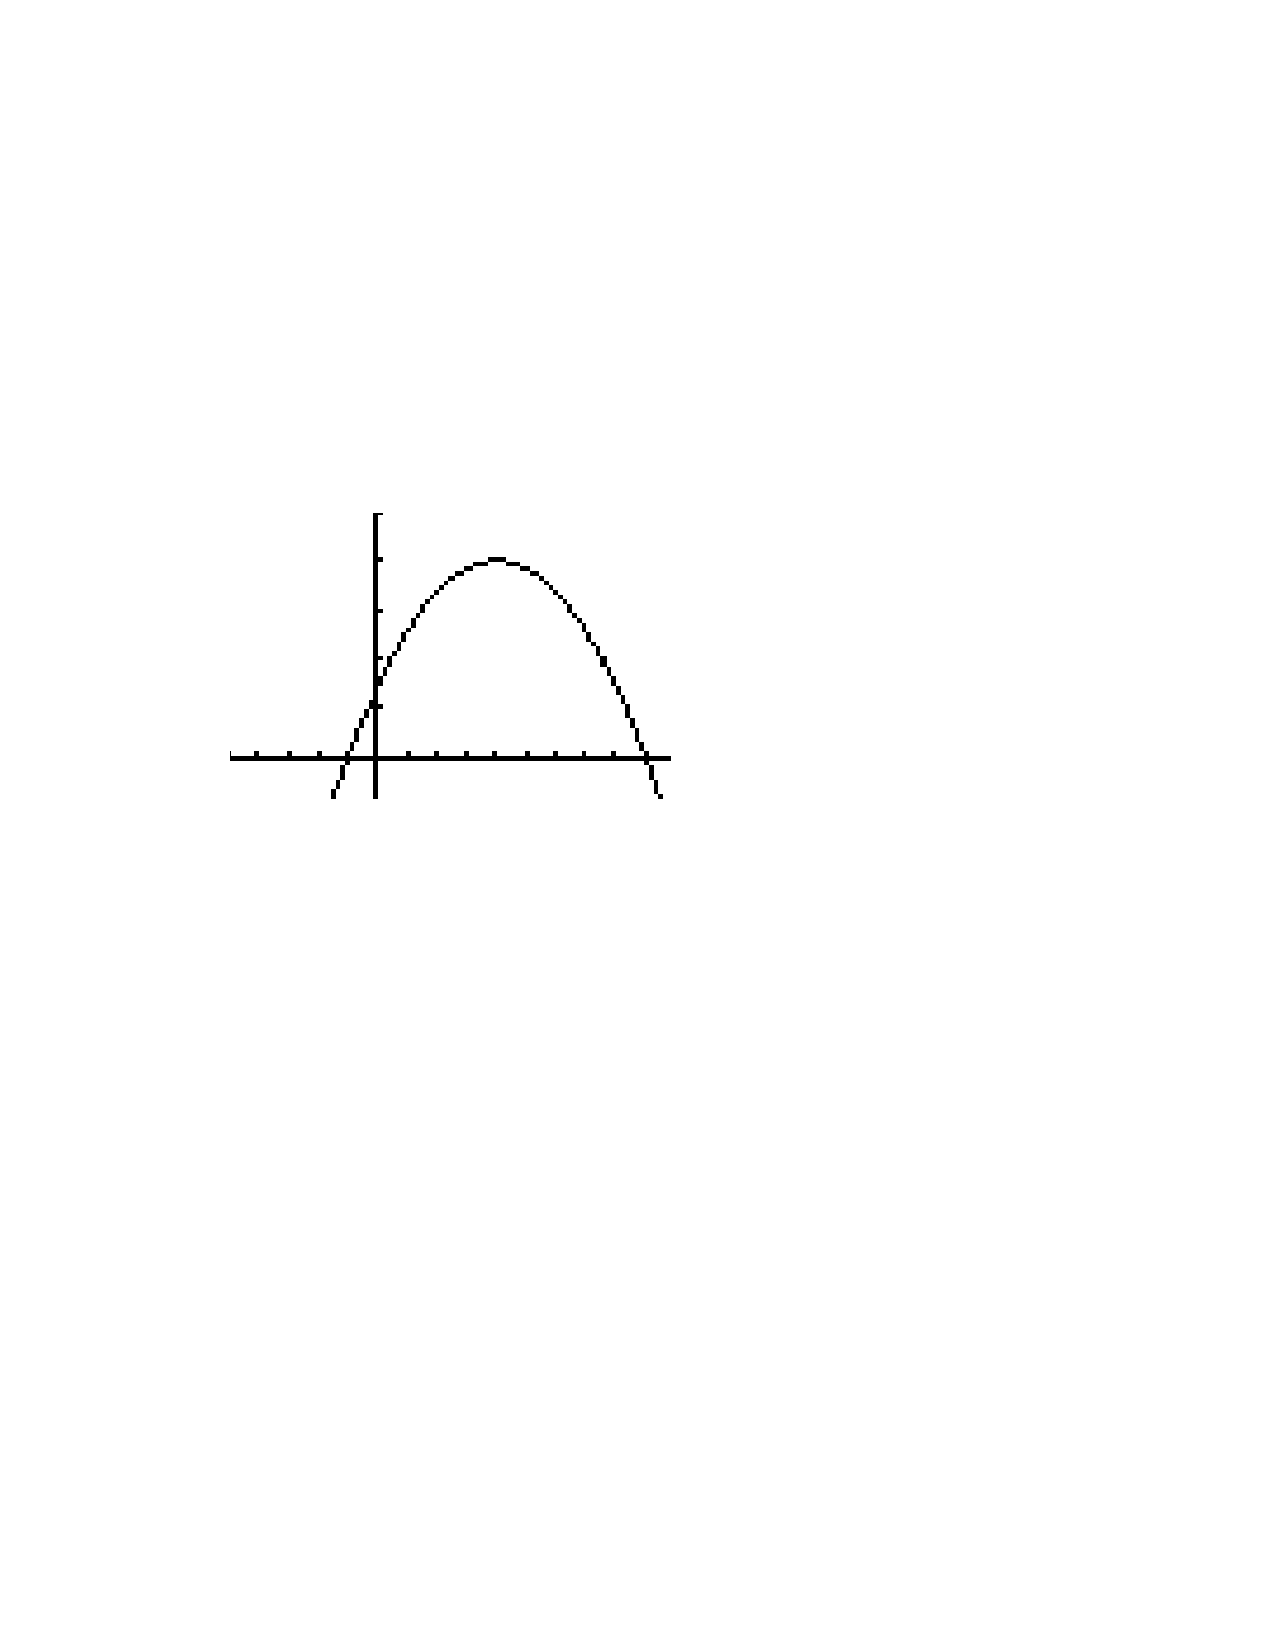
\includegraphics[trim= 250 360 300 185]{Images/Figure1.pdf}
  \end{center}
\end{problem}

\begin{problem}
  \label{problem:find-all-asymptotes}
  For the function $g$ defined by 
  \[
    g(t) = \frac{t^2 + 7t + 11}{t-3}
  \]
  \begin{itemize}
    \item[(a)]
      Find all vertical asymptotes, (be sure to mention how the function approaches its vertical asymptotes).

    \item[(b)]
      Find all horizontal asymptotes.

    \item[(c)]
      Find all slant asymptotes.
  \end{itemize}
\end{problem}

\subsection*{Extra Problems for for Personal Practice}
\label{section:extra-problems}
\begin{problem}
  \label{problem:briggs-2-5-69}
  Find the vertical and horizontal asymptotes of
  \[
    f(x) = \frac{\cos(x) + 2\sqrt{x}}{\sqrt{x}}.
  \]
\end{problem}

\begin{problem}
  \label{problem:briggs-2-5-82}
  Use the following instructions to evaluate the given limits of
  \[
    f(x) = \frac{e^x + e^{2x}}{e^{2x} + e^{3x}}.
  \]
  \begin{itemize}
    \item[(a)]
      Evaluate $\displaystyle \lim_{x \to \infty} f(x)$ be dividing both numerator and denominator by $e^{3x}$.

    \item[(b)]
      Evaluate $\displaystyle \lim_{x \to -\infty} f(x)$ be dividing both numerator and denominator by $e^{2x}$.

    \item[(c)]
      Give the horizontal asymptote(s).

    \item[(d)]
      Graph $f$ and confirm your work in parts (a)--(c).
  \end{itemize}
\end{problem}

\begin{problem}
  \label{problem:asymptotes}
    For each of the given functions:
  \begin{itemize}
    \item
      find all vertical asymptotes, (be sure to mention how the function approaches its vertical asymptotes)
    \item
      find all horizontal asymptotes,
    \item
      if any, find all points where the function intersects its vertical asymptotes, and
    \item
      if any, find all points where the function intersects its horizontal asymptotes.
  \end{itemize}
  \begin{itemize}
    \item[(a)] The function $f$ defined by $\displaystyle f(x) = \frac{\sqrt{2x^2 + 1}}{3x-5}$.

    \item[(b)] The function $s$ defined by $\displaystyle s(t) = \sqrt{t^2 + 8t + 1} - t$.
  \end{itemize}
\end{problem}

\begin{problem}
  \label{problem:sketch-a-graph}
  Sketch the graph of a function that satisfies all of the given properties.
  (You \emph{do not} need to find a formula for the function.)

  \begin{center}
    \begin{tabular}[c]{llll}
      \toprule
      & & \hspace{-5em}Required Properties\\
      \midrule
      $\displaystyle \lim_{x \to -2^-} f(x) = \infty$ & $f(-2) = 7$ & $f(1) = 2$ & $\displaystyle \lim_{x \to \infty} f(x) = 3$ \\
      $\displaystyle \lim_{x \to -\infty} f(x) = -\infty$ & $\lim_{x \to 5} f(x) = \infty$ & $\displaystyle \lim_{x \to 9} f(x) = 3$ & $f(9) = 1$\\
      $\displaystyle \lim_{x \to -3^-} f(x) = \infty$ & $\displaystyle \lim_{x \to -3^+} f(x) = -\infty$ & $f(4) \text{ is undefined, }$ & $f(x) = 3 \text{ for } x>9$\\
      \bottomrule
    \end{tabular}
  \end{center}
\end{problem}
\end{document} 
